\section{Moderation of effects by individual characteristics}\label{ssec:moderationeffects}

In~\cite{olguinmunoz2021impact}, we recorded variables related to well-known individual differences, encompassing both the \glspl{BFI}~\cite{john1999big}, and the \glspl{ITQ}~\cite{witmer1998measuring}.
Out of the individual-difference variables, the most salient effect on performance corresponded to \emph{neuroticism}, a \gls{BFI} trait linked to low tolerance for stress and high emotional reactivity, and which has previously been linked to higher \emph{delay discounting} rates~\cite{hirsh2008delay}.
Delay discounting is the tendency to devalue rewards for which one must wait; high rates, indicative of waiting intolerance, have been associated with negative social and academic outcomes.

% Bobby suggested we remove this figure and just give the pearson coeff.
% \begin{figure}
%     \centering
%     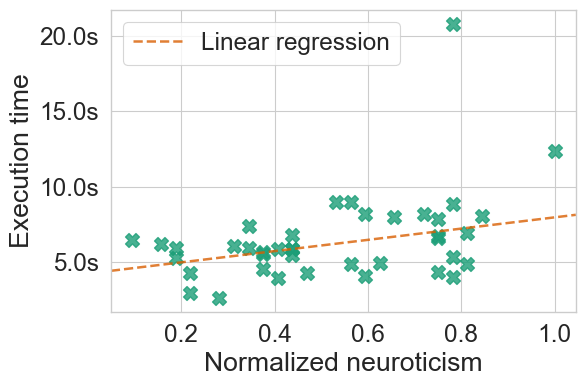
\includegraphics[width=\textwidth]{figs/new_model/correlation_neuro_exectime.png}
%     \caption{%
%         Correlation between neuroticism and the mean execution time of the last four steps in segments of \num{12} steps subject to the same \gls{TTF} in~\textcite{olguinmunoz:impact2021}.
%         Pearson correlation coefficient \( \rho = 0.418 \), 2-tailed \( p < 0.05 \).
%     }\label{fig:neuroexectimecorrel}
% \end{figure}

% In this work, we have used a normalized scale to describe neuroticism, derived from the minimum and maximum obtainable values for this variable in the \gls{BFI}~\cite{john1999big}.
% \emph{Low} and \emph{high} neuroticism refer to the \( [0.0, 0.5) \) and \( [0.5, 1.0] \) ranges respectively.

Linear regression showed a significant correlation between individual neuroticism scores and the execution time late in a series of high-delay steps, \( \rho = 0.418 \), \num{2}-tailed \( p < 0.05 \)
Neuroticism was further identified as a modulating factor for the pacing effects through a \gls{PCA}.
Out of the three identified components, which cumulatively accounted for \SI{73.13}{\percent} of the variance in the results, neuroticism was included in the first two.
The effect of neuroticism was observed across all \glspl{TTF} and impairment durations in the tasks.

Furthermore, we found that execution times, when grouped by experimental variables such as neuroticism, \gls{TTF}, and continuous segments of steps subject to the same \gls{TTF}, were well-fit by an \gls{exGaussian} distribution, as verified using Kolmogorov-Smirnov goodness-of-fit tests~\cite{massey_jr1951kolmogorov}.
When grouping by level of neuroticism, \gls{TTF}, and \emph{slice}\footnote{%
In~\cite{olguinmunoz2021impact} the \emph{slice} to which a step belongs to refers to whether the step occurred in the first, second, or third four-step segment of a sequence of steps subject to the same \gls{TTF}.
}, the best fit statistic was \ensuremath{0.028} (\ensuremath{p = 0.999}).
This distribution has an ample body of research supporting its suitability for the modeling of the timing of human actions and reaction times~\cite{rohrer1994analysis,palmer2011what,marmolejo_ramos2022generalised}.
We found that the effects of neuroticism on execution times were clearly identifiable in the fitted distributions, in particular in their means and tails.
\cref{fig:muexgaussian} shows an example of this modulating effect, illustrating the behavior of the mean (\( \mu \) parameter) of \gls{exGaussian} distributions fitted to the execution times of the first four steps of segments of steps subject to the same \gls{TTF}.
Finally, \cref{fig:fitsneuro} shows an example of the effects of neuroticism on the fitted \gls{exGaussian} distributions for a specific group of execution times.
Higher neuroticism directly translates into a higher mean and longer tail.

\begin{figure}
    \centering
    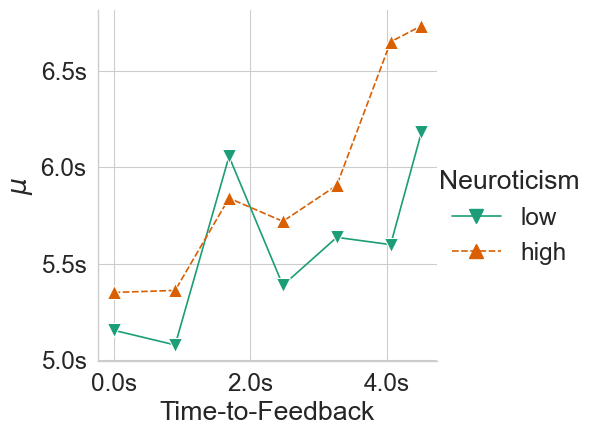
\includegraphics[width=.9\columnwidth]{figs/new_model/mu_fits_exgaussian_slice0}
    \caption{%
        \( \mu \) parameter of \gls{exGaussian} distributions fitted to execution times of the first four steps of segments of steps subject to the same \gls{TTF} in~\cite{olguinmunoz2021impact}.
        Distributions were fitted using \gls{MLE}.
    }\label{fig:muexgaussian}
\end{figure}

\begin{figure}
    \centering
    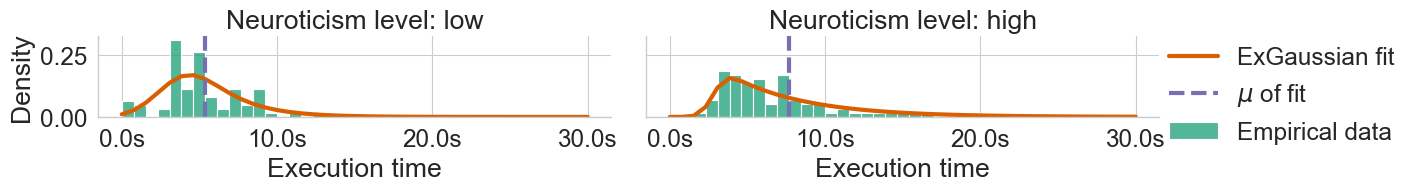
\includegraphics[width=.9\columnwidth]{figs/new_model/dist_fits_neuro}
    \caption{%
        Example \gls{exGaussian} fits on execution times from steps \numrange{4}{8} in a segment of steps at the maximum experimental \gls{TTF}.
        The effects of neuroticism are clearly visible in the tail and the mean of the distributions.
    }\label{fig:fitsneuro}
\end{figure}.